\chapter{Supplementary Material}
\label[appsec]{chap:supplementary_computations_and_proofs}
\section{Mathematical Foundation of Machine Learning}
\subsection{Mean Squared Error Loss and Conditional Expectation}
\label[appsec]{app:mse_mean}
When performing a minimisation of the batch loss based on the mean squared error (MSE) in a supervised learning setting, one can show that the optimal predictor corresponds to the conditional expectation of the target variable given the input features.
The MSE batch loss can be written as:
\begin{equation}
  \mathcal{L}_{\text{MSE}}(f_{\boldsymbol{\theta}}) = \frac{1}{N}
  \sum_{i=1}^{N} (\mathbf{y}_i - f_{\boldsymbol{\theta}}(\mathbf{x}_i))^2~.
\end{equation}
Using a simple calculus argument, one can show that the function $f_{\boldsymbol{\theta}}$ that minimises this batch loss is given by:
\begin{align}
  \frac{d}{d{\boldsymbol{\theta}}} \mathcal{L}_{\text{MSE}}(f_{\boldsymbol{\theta}}) & = \frac{d}{df} \int (\mathbf{y} - f_{\boldsymbol{\theta}}(\mathbf{x}))^2 p(\mathbf{y}|\mathbf{x}) \,d\mathbf{y} \cdot \frac{\partial f}{\partial {\boldsymbol{\theta}}}   \\
  & = \int 2(f_{\boldsymbol{\theta}}(\mathbf{x}) - \mathbf{y}) p(\mathbf{y}|\mathbf{x}) dy \cdot \frac{\partial   f}{\partial {\boldsymbol{\theta}}}\overset{!}{=} 0 \\
  \Rightarrow f_{\boldsymbol{\theta}}(\mathbf{x})
  & = \int \mathbf{y} p(\mathbf{y}|\mathbf{x}) \,d\mathbf{y} = \mathbb{E}_{\mathbf{y}|\mathbf{x}}(\mathbf{y})~.
\end{align}

\subsection{Equivalence of Maximum Likelihood and KL-Divergence Minimisation}
\label[appsec]{app:ml_kld}
Let $p_{\text{data}}(\mathbf{x})$ denote the true data distribution and $p_{\boldsymbol{\theta}}(\mathbf{x})$ a parametric model. The KL-divergence between them is defined as 
\begin{equation}
  D_{\text{KL}}(p_{\text{data}} \| p_{\boldsymbol{\theta}})
  = \mathbb{E}_{\mathbf{x} \sim p_{\text{data}}} \left[ \log
  \frac{p_{\text{data}}(\mathbf{x})}{p_{\boldsymbol{\theta}}(\mathbf{x})} \right]
  = \mathbb{E}_{\mathbf{x} \sim p_{\text{data}}} \left[ \log p_{\text{data}}(\mathbf{x}) \right]
  - \mathbb{E}_{\mathbf{x} \sim p_{\text{data}}} \left[ \log p_{\boldsymbol{\theta}}(\mathbf{x}) \right].
\end{equation}
Since the first term, $-H(p_{\text{data}})$, is the negative entropy of the data distribution and does not depend on ${\boldsymbol{\theta}}$, minimising the KL-divergence over ${\boldsymbol{\theta}}$ is equivalent to \begin{equation}
  \hat{{\boldsymbol{\theta}}} = \argmin_{\boldsymbol{\theta}} D_{\text{KL}}(p_{\text{data}} \| p_{\boldsymbol{\theta}})
  = \argmax_{\boldsymbol{\theta}} \, \mathbb{E}_{\mathbf{x} \sim p_{\text{data}}} \left[ \log
  p_{\boldsymbol{\theta}}(\mathbf{x}) \right].
\end{equation}
Approximating the expectation over $p_{\text{data}}$ by the empirical mean over a dataset $\{x_i\}_{i=1}^{N}$ of $N$ independent observations gives \begin{equation}
  \hat{{\boldsymbol{\theta}}} = \argmax_{\boldsymbol{\theta}} \frac{1}{N} \sum_{i=1}^{N} \log
  p_{\boldsymbol{\theta}}(\mathbf{x}_i),=\argmin_{\boldsymbol{\theta}} \frac{1}{N} \sum_{i=1}^{N} -\log p_{\boldsymbol{\theta}}(\mathbf{x}_i)
\end{equation}
which is precisely the maximum likelihood estimator. Note that this simply generalises to the case of a conditional probability.

\subsection{Gaussian-Loss as Minimisation of the KL-divergence}
\label[appsec]{app:gaussian_loss}
Assume the conditional parametric model to have the form of a (multidimensional) Gaussian distribution,
\begin{equation}
  p_{\boldsymbol{\theta}}(\mathbf{y}|\mathbf{x})=\prod_i^{\text{dim}}\frac{1}{\sqrt{2\pi\sigma_{i,{\boldsymbol{\theta}}}^2(\mathbf{x})}}\exp\left(-\frac{(y_i-\mu_{i,{\boldsymbol{\theta}}}^2(\mathbf{x}))^2}{2\sigma_{i,{\boldsymbol{\theta}}}^2(\mathbf{x})}\right)~.
\end{equation}
For this, one can now consider the negative log-likelihood (NLL) of a dataset of $\{x_j\}_{j=1}^{N}$ of $N$ independent observations:
\begin{align}
  \text{NLL}(p_{\boldsymbol{\theta}})&=\frac{1}{N}\sum_{j=1}^N-\log(p_{\boldsymbol{\theta}}(\mathbf{y}|\mathbf{x}))\\
  &=\frac{1}{N}\sum_{j=1}^N\sum_{i=1}^{\text{dim}}\left(\frac{1}{2}\log(2\pi)+\frac{1}{2}\log(\sigma_{i,{\boldsymbol{\theta}}}^2(\mathbf{x}))+\frac{(y_i-\mu_{i,{\boldsymbol{\theta}}}^2(\mathbf{x}))^2}{2\sigma_{i,{\boldsymbol{\theta}}}^2(\mathbf{x})}\right)~.
\end{align}
The constant term $\log(2\pi)$ can be dropped for the minimisation, which results in \begin{align}
  \hat{\boldsymbol{\theta}}&=\argmin_{\boldsymbol{\theta}} \text{NLL}(p_{\boldsymbol{\theta}})\\
  &=\argmin_{\boldsymbol{\theta}} \frac{1}{N}\sum_{j=1}^N\sum_{i=1}^\text{dim}\left(2\log(\sigma_{i,{\boldsymbol{\theta}}}(\mathbf{x}))+\frac{(y_i-\mu_{i,{\boldsymbol{\theta}}}^2(\mathbf{x}))^2}{\sigma_{i,{\boldsymbol{\theta}}}^2(\mathbf{x})}\right)~.
\end{align}

\section{Neutrino Momenta Posterior Distributions}
\label[appsec]{app:neutrino_probs}
\subsection{Invariant Mass of Top-Quark Pair}
\begin{figure}[H]
  \centering
  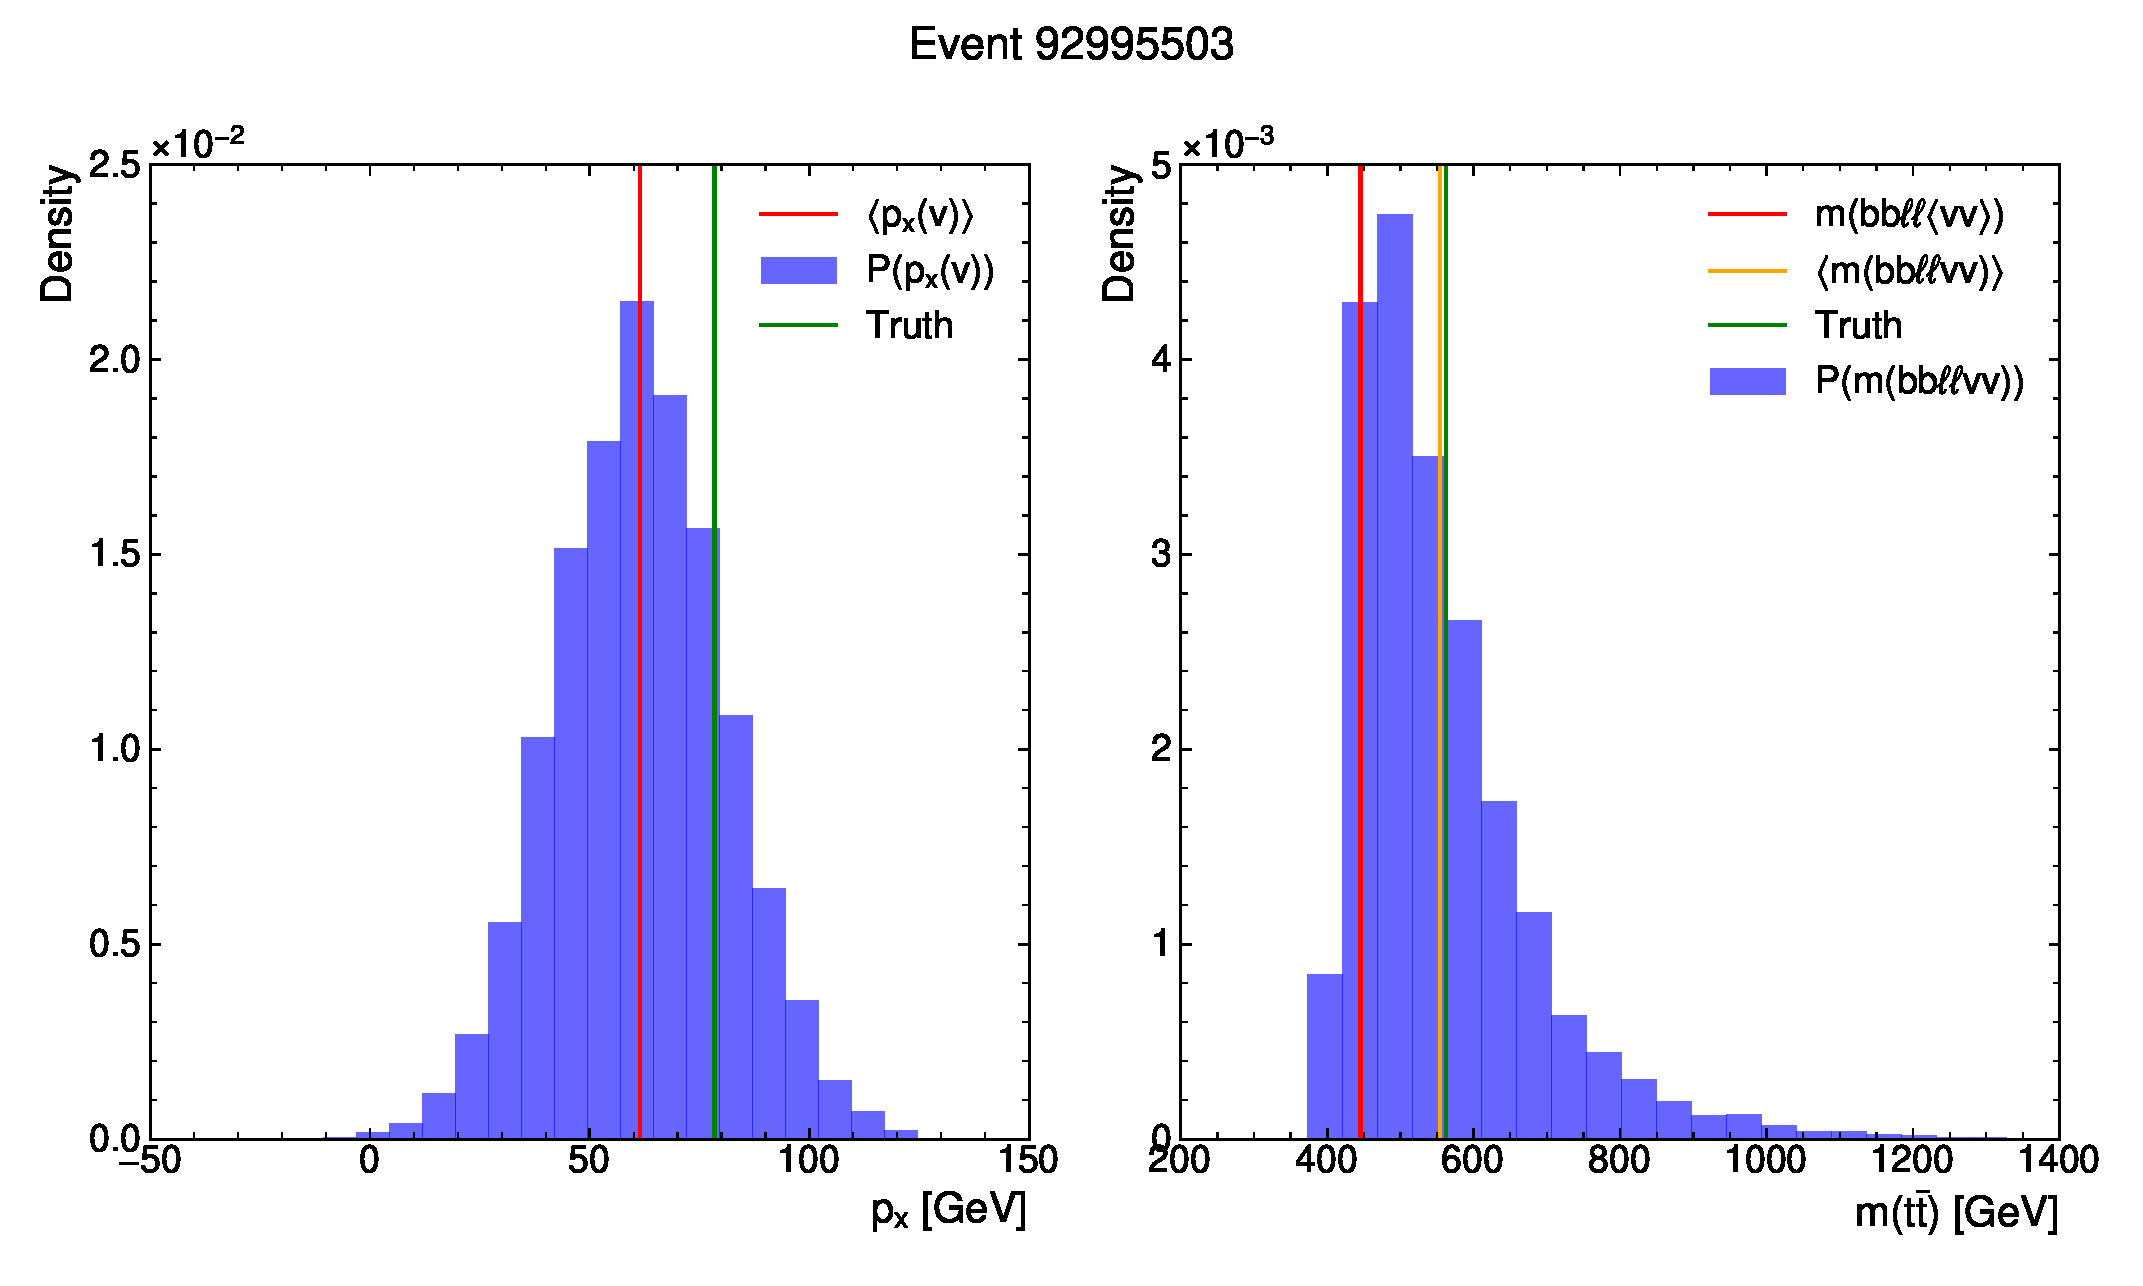
\includegraphics[width=1.0\textwidth]{plots/gaussian_loss_plots/gaussian_loss_sample_mttbar_plots.pdf}
  \caption{Plots showing the probability distribution of the neutrino momentum component $p_x$ and the reconstructed invariant mass $m(t\bar{t})$ based on the mean and standard deviation predicted by the MMT-model trained with a Gaussian-loss for a random event.}
  \label{fig:gaussian_loss:mttbar_posterior_sample}
\end{figure}


\subsection{Spin-Sensitive Variable \chel}
\begin{figure}[H]
  \centering
  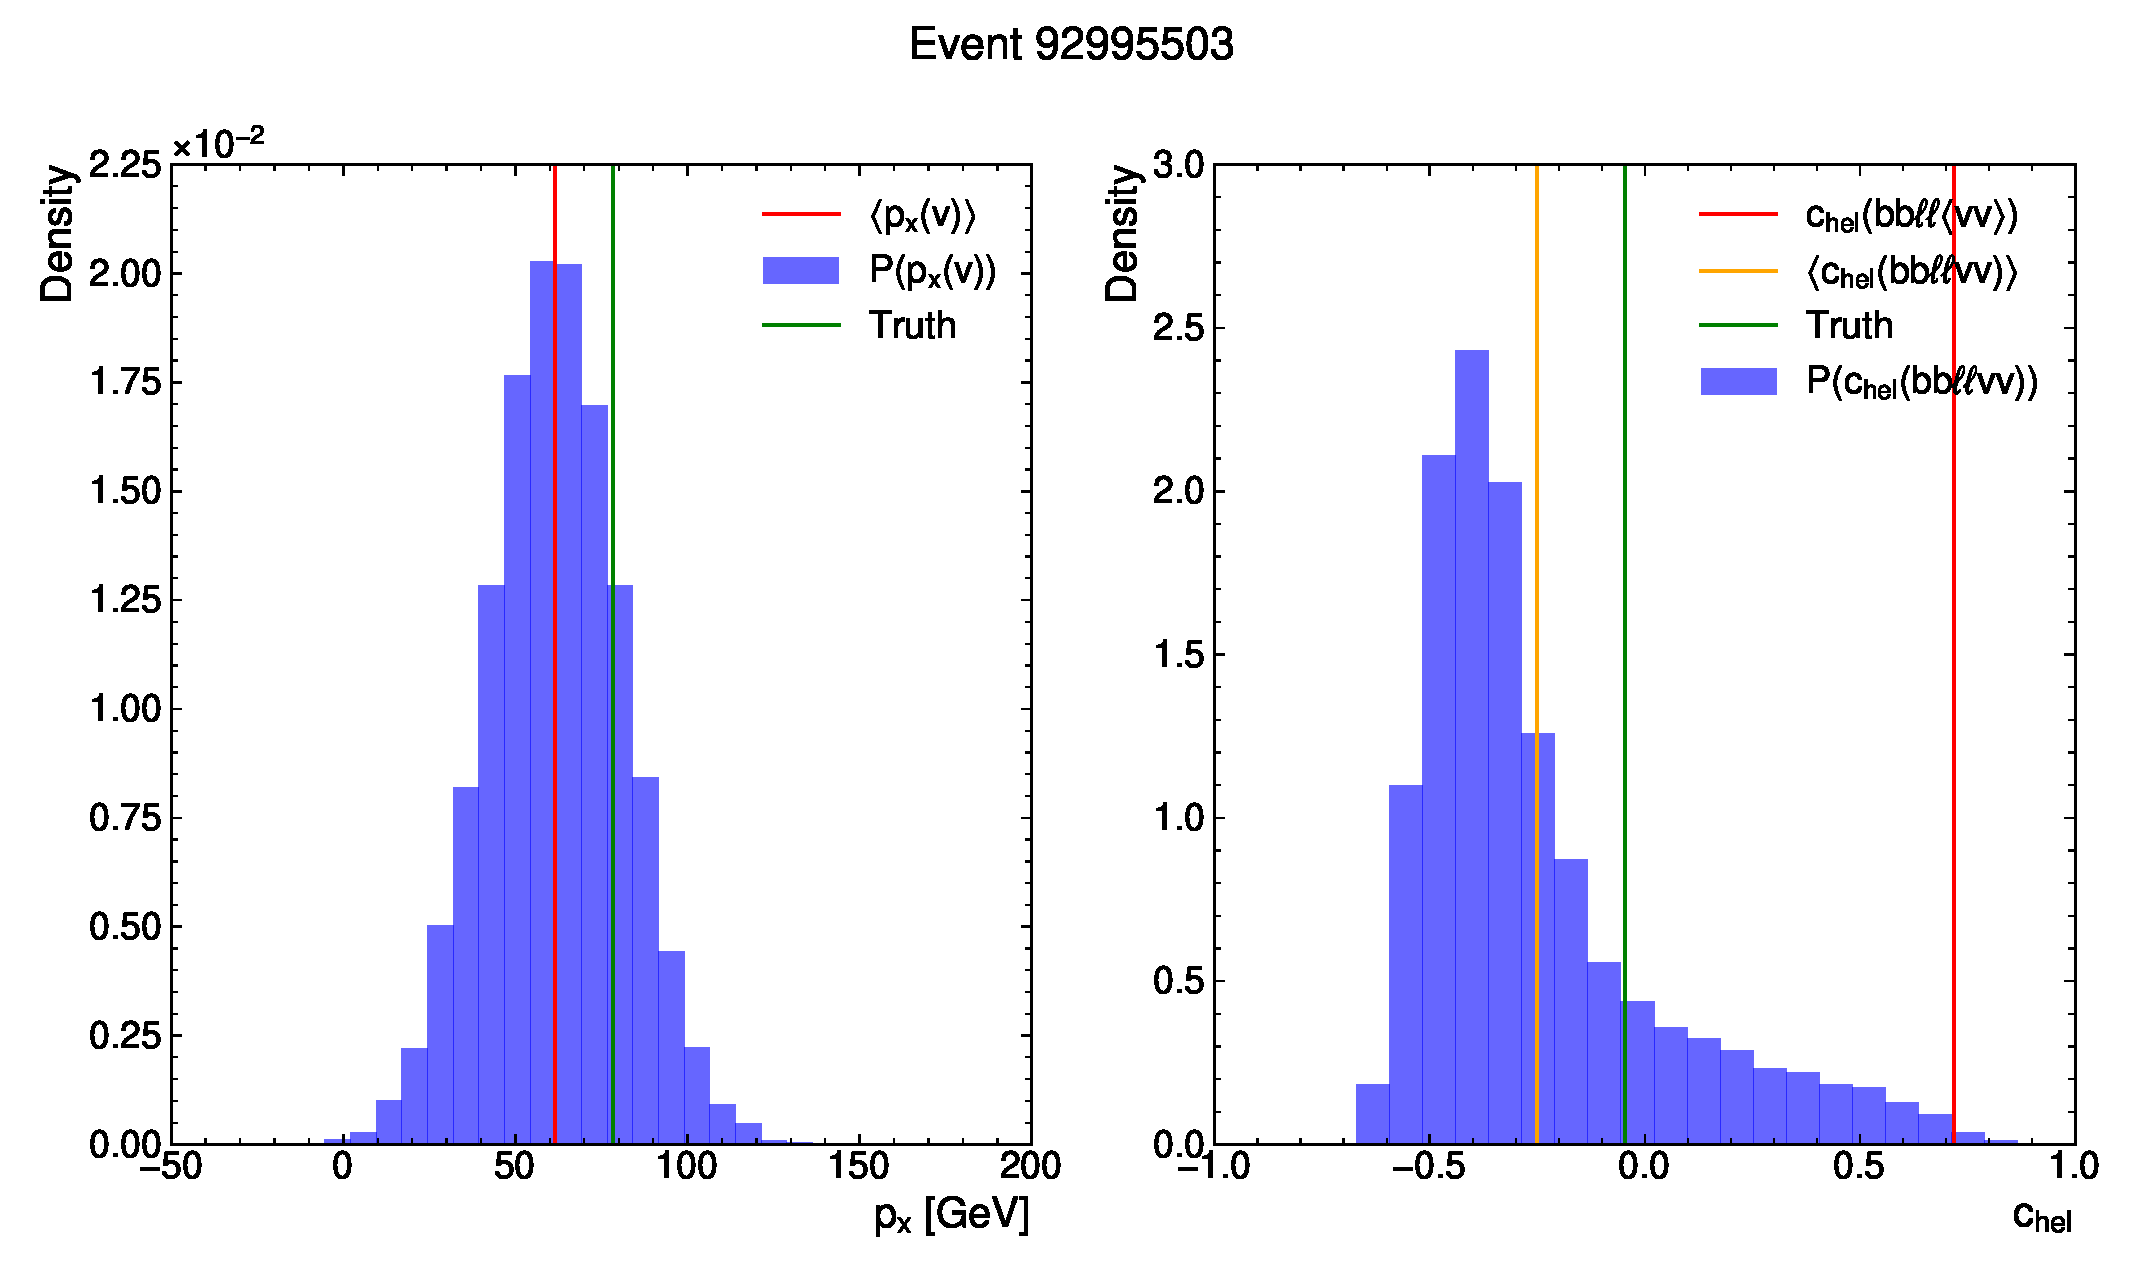
\includegraphics[width=1.0\textwidth]{plots/gaussian_loss_plots/gaussian_loss_sample_c_hel_plots.pdf}
  \caption{Plots showing the probability distribution of the neutrino momentum component $p_x$ and the reconstructed \chel based on the mean and standard deviation predicted by the MMT-model trained with a Gaussian-loss for a random event. Indicated are the mean and true values by vertical lines.}
  \label{fig:gaussian_loss:c_hel_posterior_sample}
\end{figure}
\begin{figure}[H]
  \centering
  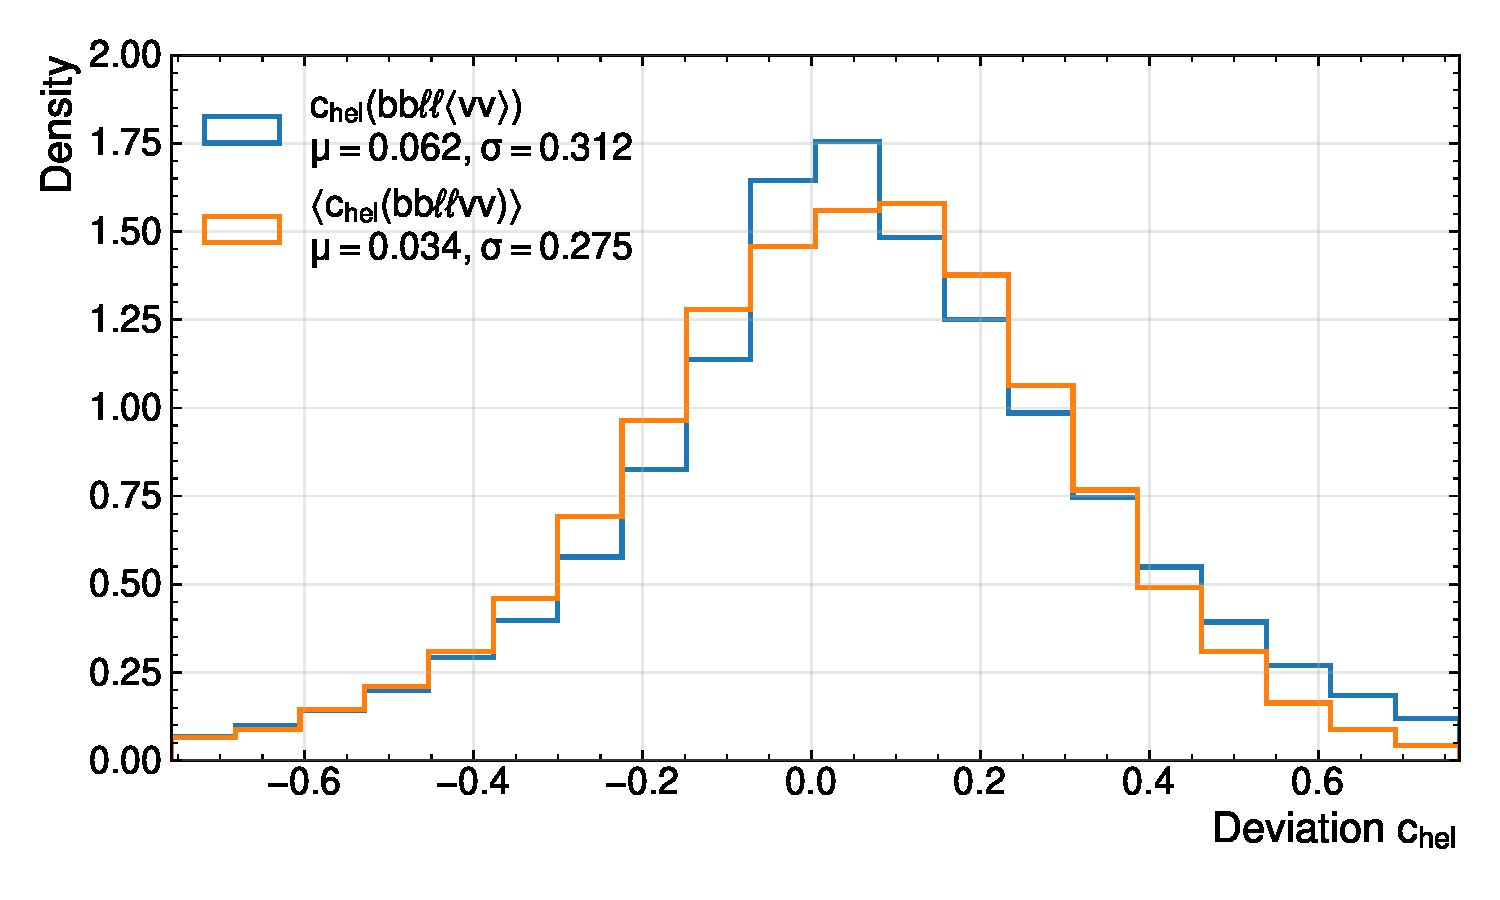
\includegraphics[width=0.7\textwidth]{plots/gaussian_loss_plots/gaussian_loss_c_hel_posterior_deviation.pdf}
  \caption{Deviation between the reconstructed and true \chel. The different curves show, whether the invariant mass was computed using the mean momentum or by propagating the neutrino probabilities and averaging of the obtained spin-variable.}
  \label{fig:gaussian_loss:c_hel_posterior_deviation}
\end{figure}

\subsection{Spin-Sensitive Variable \chan}
\begin{figure}[H]
  \centering
  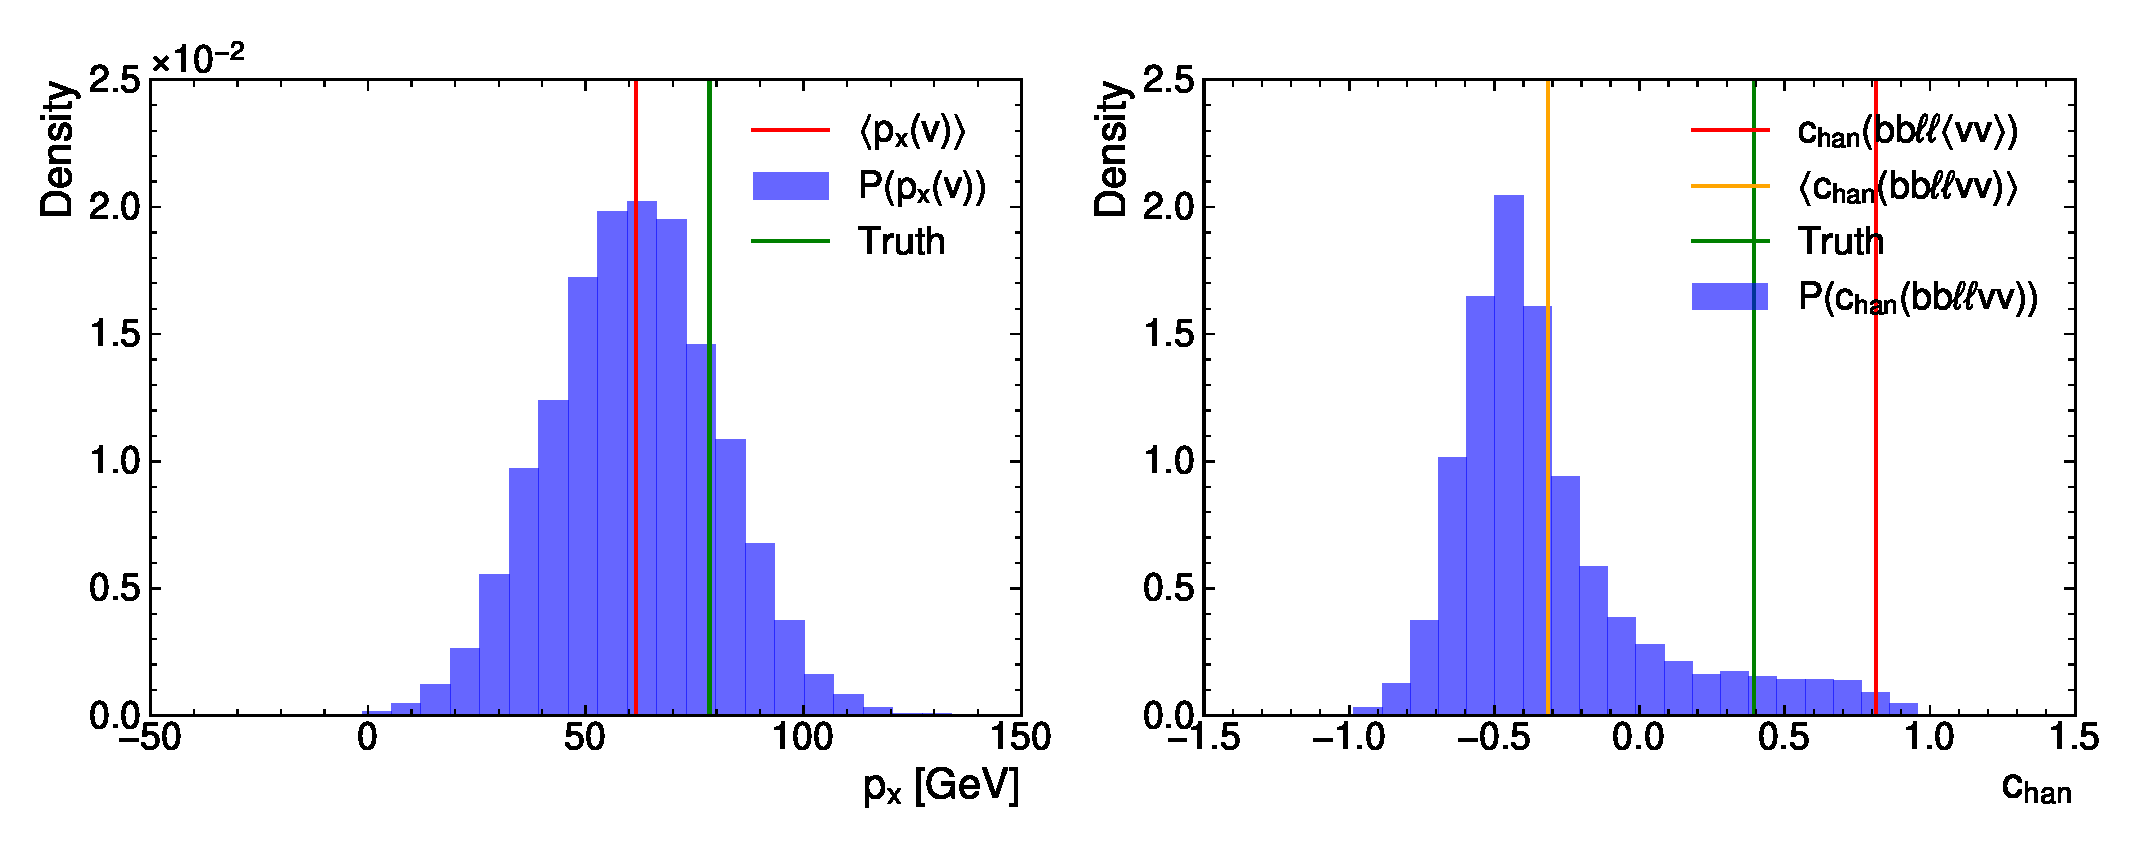
\includegraphics[width=1.0\textwidth]{plots/gaussian_loss_plots/gaussian_loss_sample_c_han_plots.pdf}
  \caption{Plots showing the probability distribution of the neutrino momentum component $p_x$ and the reconstructed \chan based on the mean and standard deviation predicted by the MMT-model trained with a Gaussian-loss for a random event. Indicated are the mean and true values by vertical lines.}
  \label{fig:gaussian_loss:c_han_posterior_sample}
\end{figure}
\begin{figure}[H]
  \centering
  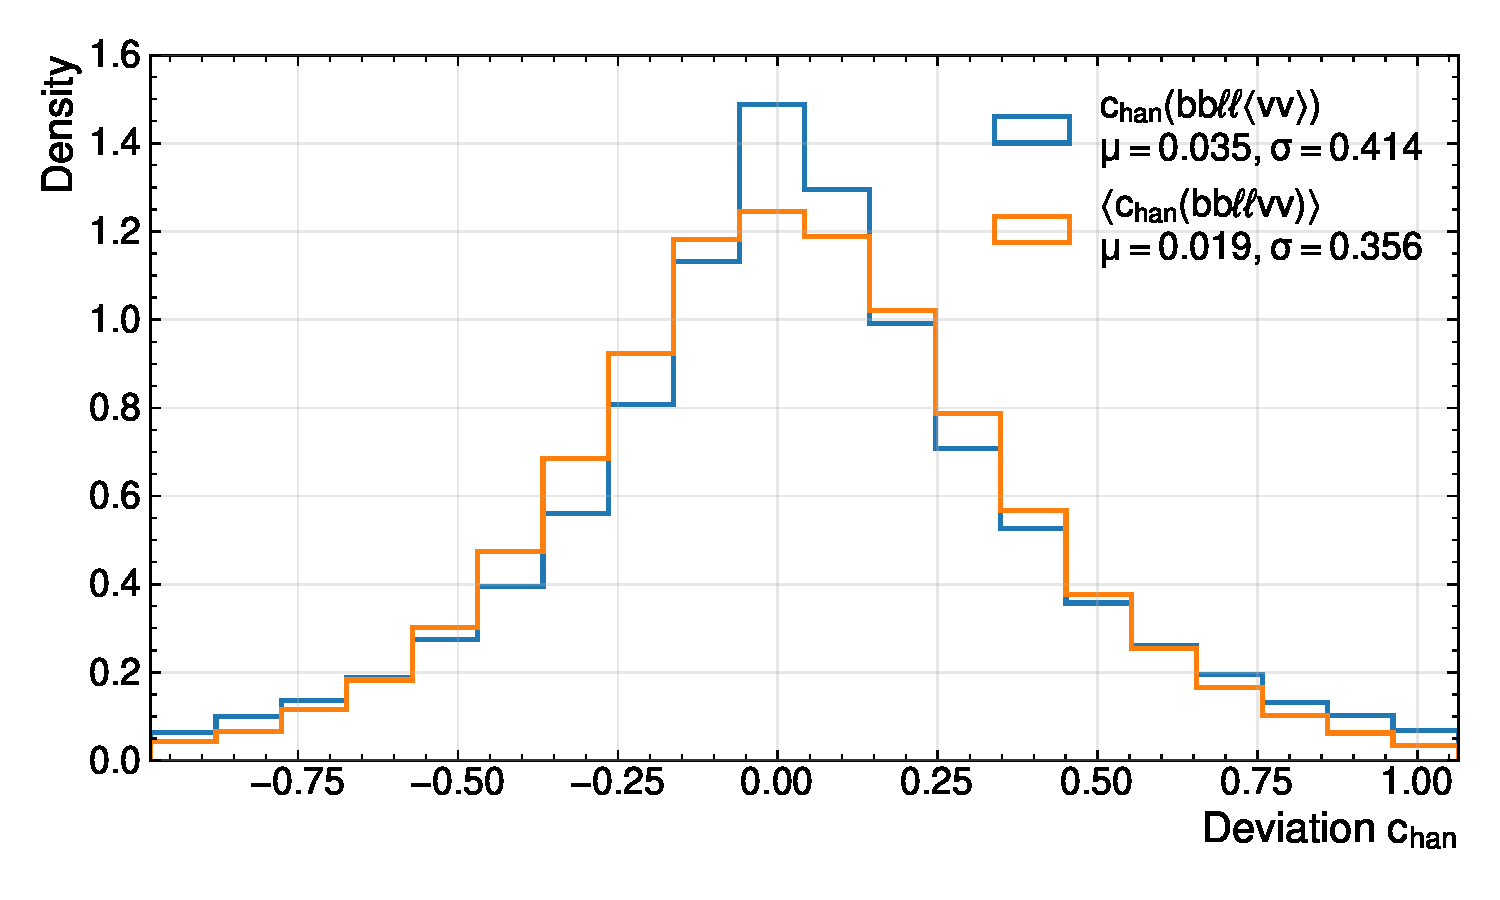
\includegraphics[width=0.7\textwidth]{plots/gaussian_loss_plots/gaussian_loss_c_han_posterior_deviation.pdf}
  \caption{Deviation between the reconstructed and true \chan. The different curves show, whether the invariant mass was computed using the mean momentum or by propagating the neutrino probabilities and averaging of the obtained spin-variable.}
  \label{fig:gaussian_loss:c_han_posterior_deviation}
\end{figure}
